\documentclass[10.5pt]{article}
\usepackage{uspstyle}
\usepackage{graphicx}
\usepackage{mathrsfs}
\usepackage{amsfonts}
\begin{document}





% The content of your research proposal, including text, figures and images, 
% should not exceed 5 pages, typed, double-spaced (additional pages may be 
% included for your works-cited/references).
\section*{Model Testing using Topological Data Analysis - Ryan Hansen}

\section{Introduction}
% Provide a statement of the objective(s) and the anticipated significance of the 
% work to your field of study. What problems will be investigated? What hypothesis 
% will be tested? We suggest that the introduction begin with a brief description 
% of the project in general terms before the more technical aspects of the project 
% are discussed. 
%\todo{put some sort of high-level introduction here.}
%here is how you cite a figure (be sure to updated the ref here ... and the 
%label inside the figure

Our goal as scientists is to create predictory models. We want to completely understand phenomena so we can use what we know to solve problems. The way we see if these models are reliable is through vigorous comparison to data. This becomes an issue when data isn't very reliable. Biological data, the primary focus of our project, is often subject to high levels of variability \cite{bionoise}. In many scenarios, data collection methods lead to significant sources of error, for example, when sampling from multiple tissues or organisms. Our goal is to resolve this inherent inconsistency through the scope of Topological Data Analysis, (TDA), whose framework provides several advantages. TDA provides many tools that work remarkably well on high dimensional, high noise data \cite{robinson2017sheaves}. One of these tools is called a sheaf, which can be used to quantify how consistent any given predictive model is with its corresponding data. If they do not agree, sheaf structure can account for components of a given model that may have been previously excluded. This is a powerful tool for high dimensional data and model testing, since it not only suggests if our model is lacking, but also indicates what parameters are responsible for the model and data diverging. We are particularly interested in applying this idea to metabolomics, whose data is collected from several sources of differing cells and/or individuals. As a high dimensional system of stoichiometric equations (linear in nature) subject to high levels of variability, metabolomics is an ideal gateway to studying how to apply the sheaf consistency framework to real world models.
%Figure~\ref{fig:TODO-name}

%TO cite something, use~\cite{fasy2014statistical}.

% \begin{figure}
%  \centering
%  \includegraphics[height=1.25in]{TODO:relative-path}
%  \caption{TODO.}\label{fig:TODO-name}
% \end{figure}

\section{Background}
% Provide a brief review of the work that has been done in the project 
% area together with complete references in appropriate professional style. This 
% section should also include any personal information about you that would 
% indicate to the reviewers your qualifications for successfully completing this 
% project, including a statement of how the project will contribute to your 
% academic and career goals.
%\todo{discuss related work, and why you are qualified to work on this.  Perhaps 
%make subsections.}
\subsection{What is TDA and why is it advantageous}
TDA, Topological Data Analysis, is the process of using topological descriptors to derive meaning from data. Suppose we have two different pictures of a bunny. Most everyone can tell the pictures are both bunnies. Now suppose we tell a computer one of them is a bunny. The computer has a very hard time identifying the second image as a bunny. This is where TDA is advantageous. Despite moving a leg or wiggling an ear, topologically, the bunnies are equivalent. It is this versatility that is useful in many situations of data analytics. In our scenario we define a topology on the mathematical model we are testing, the system of stoichiometric equations. The inherent permitted variability in all topological equivalences is useful while studying the accuracy of our model for two reasons. First, we permit slight errors in the model. We expect some error in all situations given how many variables exist in the world. What matters most is if the core shape of the data matches what we expect is correct. Second, if the core model does not match the shape of the data, topology gives us enough information to attempt to amend the presumably flawed model. For our project, this is realized through sheaves, which will be covered more thoroughly in the methods section.

\subsection{Personal Value}
I am a Physics and Computer Science major who also enjoys math. Being involved in TDA at MSU during my undergraduate degree is extremely beneficial to me. I get the opportunity to learn an incredible amount of material, I get to work with fantastic and intelligent people, I get to enhance my public speaking and presentation skills, I learn techniques for high quality technical writing, and lastly, it prepares me for future vocation. All of these things will help secure a job and a position in graduate school, of which I am aspiring for both. 
\subsection{Qualifications}
I have been a part of the TDA group since early 2018. As such, I have built the foundations for doing research in the field, including participating in the spring semester of the course "Computational Topology," and in the group's summer and fall reading sessions. In addition, I have worked on this problem in the past and am already familiar with the subject.


\section{Methods}
% Provide a detailed description of the research methods that you will 
% use in the project. This should include a justification for the specific 
% approach that you will use. For example, how do the methods answer the questions 
% that have been posed, test the hypothesis, or lead to the desired goal?
% Timeline: Provide dates for the initiation and completion of each phase of the 
% project. Attempt to lay out a reasonable schedule taking into consideration all 
% phases of the research and final deliverables.

As commonly denoted, let the sheaf $\mathscr{F}$ be a
contravariant functor. Our goal is to apply the tools of a sheaf to metabolic data in order to handle the high-noise and high-dimensional issues it brings. As it is a functor, we must first define the category in the domain of the sheaf, the
category of reactions, $\mathcal{X}$. Then, we describe a mapping from the
objects and morphisms of $\mathcal{X}$ into the category in the image of the
sheaf functor, which we denote by $E$, a category of real Euclidean spaces. 

\subsection{The Category of Reactions}
As mentioned earlier, metabolic reactions are currently modeled as a set $\mathcal{R}$ of stoichiometric equations. Each of these equations contains a set of reactants, $M_0$, a set of products, $M_1$. Collectively, these are the objects of this category. Additionally, our model quantifies how the reactants change to products. These are the morphisms. Each reaction occurs at some rate. This means over some time interval, each reaction occurs some number of times, $r_m$. Given constants to describe the morphisms, $c_i,c_j \in \mathbb{Z}^+$, these reactions are of the form \begin{equation}
r_m\sum_{m_i \in M_0} c_i m_i \rightarrow r_m\sum_{m_j \in M_1} c_j m_j .
\end{equation}  
Together, the objects (reactants and products) and morphisms (rates and constants) completely describe the category of reactions.
\subsection{$\mathscr{F}$ and its image}
$\mathscr{F}$ is a tool that transforms the initial model to something more useful to analyze. It maintains the same core structure, though, by mapping objects to objects and morphisms to morphisms. 
We want to connect our model to measurable data. This data is recorded by measured quantities of our reactant and product parameters. Given $n$ unique parameters (reactants and/or products), our data will subsequently lie in $\mathbb{R}^n$. Since we measure them one at a time, it makes sense, then, to define the mapping in a way to isolate each parameter. We do this by utilizing the reaction rate, $r_i$. We know if a reaction happens $r_i$ times, then $r_i$ sets of reactants will be lost and $r_i$ sets of products will be gained. If we follow this process throughout the entire set of reactions and arrange them based on parameter, we subsequently have a mapping from the category of reactions to $R^n$, the category of real Euclidean spaces, where our data can be realized. This is how the sheaf maps the objects of the category of reactions. When we mandate that we maintain the same structure as the initial reaction morphisms, it turns out that the mappings in the image of $\mathscr{F}$ are simply matrix multiplication of our input set of reactions.
\subsection{Consistency}
Recall our main goal is to verify if a model is consistent or not. Using the aforementioned process, we can obtain the model's space of all permitted data. If our data's shape is significantly different than what we expect, it certainly is cause for alarm. However, in these systems of linear equations, the mappings are manifestly invertible. This means we can create two sheaves - one tied to the model and its predictions and one tied to the data. This allows us to use the tool known as "consistency radius" to measure a sort of distance between each corresponding component of the sheaves. This is powerful as it allows us to see which components of the model closely agree with data, and which components may be missing key information.

\subsection{Example}
Below is an example of our sheaf applied to a simple system of equations. With the sheaf framework, we can easily determine which portions of our model are consistent with observation (green), and which are not (red). Since we know our model is consistent for reactants A and C, we can assume our error is coming from some unaccounted for factor with B or an inaccurate reaction rate r1.  
\begin{figure}[h]
	\caption{\textit{Our sheaf applied to the reactions $A + 2B\rightarrow C$ at rate r1 and $C \rightarrow A$ at rate r2}}
	
	\centering
	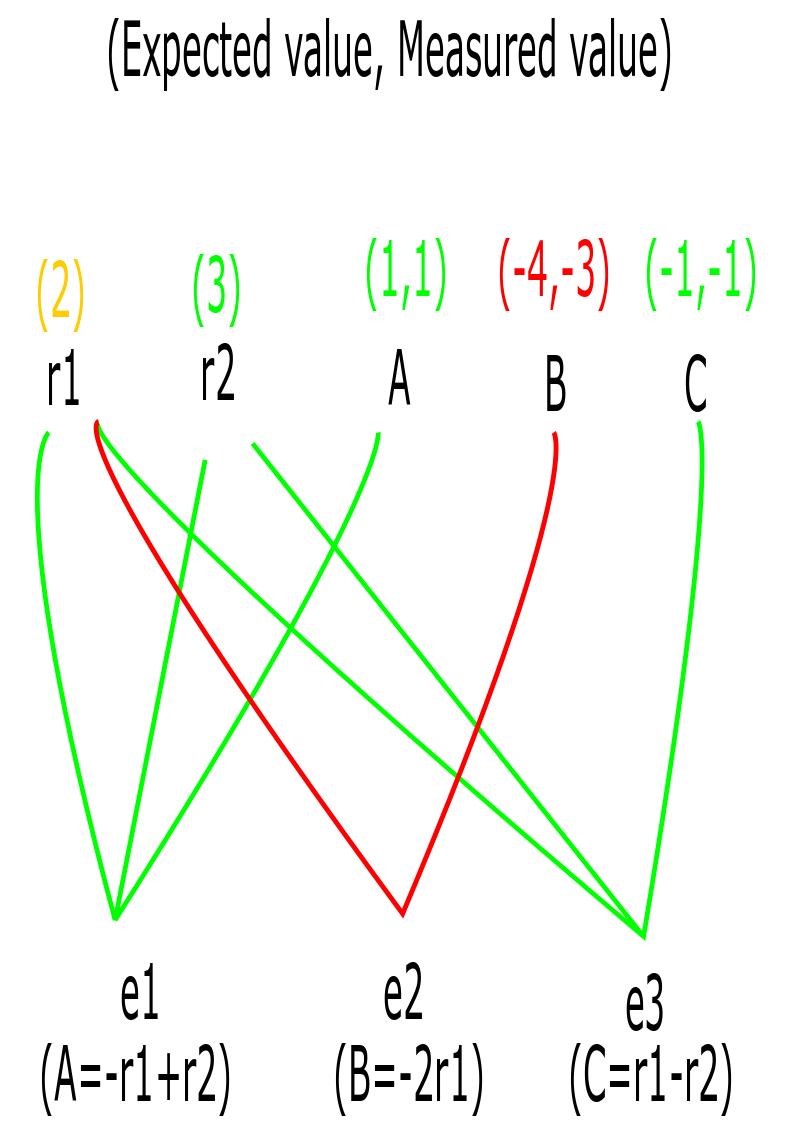
\includegraphics[width=0.5\textwidth, height=0.2\textheight]{USP2019s.PNG}
\end{figure}
\subsection{USP Goals}
We will write code that takes in, as input, a set of reactions, reaction rates, and data. It will output an indication of how well the reactions model the data.

We will verify this method of model testing using a data simulation. We will test models that have good data associated with them to show it yields acceptable responses under both consistent and inconsistent data sets.

We will write a paper explaining our process, and our findings. This paper will ideally be published, at least in MSU's research catalog.

Finally, I will create a poster presentation of my findings.
\subsection{Potential Future Related Problems}
There are a number of ways to expand this project. We can add statistical measures of confidence for determining how to accept a model. More interestingly, we want to generalize this process for data that may not have a nice linear mapping. Harder still is finding a way to analyze data that has a non invertible mapping. 
\subsection{Timeline}
January 20th - Finish core code. This code will take in the set of reactions, reaction rates, data, and output an indication of how well the reactions model the data. \\
February 10th - Finish data simulation of sufficient sample size (Consistent)\\
February 25th - Finish data simulation of sufficient sample size (Inconsistent)\\
March 3rd - Submit Abstract for Student Research Celebration\\
March 15th - Finish Poster presentation\\
April 1st - Finish paper\\
April 18th - Polished presentation and attend MSU Student Research Celebration

\section{Collaboration}
% Provide a description of the way you and 
% your faculty sponsor will collaborate on the project. The faculty sponsor should 
% play a significant role in responding to your ideas, providing advice for new 
% directions and resources, discussing the implications of the results, and 
% helping you prepare for your public presentation. Will there be regularly 
% scheduled meetings between you and your sponsor? Explain how the project relates 
% to the ongoing work of your sponsor, if this is the case.
In order to complete this project, I will be working closely with my faculty advisor, Dr. Brittany Fasy. Additionally, I will be working with Anna Schenfisch, a graduate student in mathematics, and former MSU Post-Doctoral fellow Daniel Salinas. Our group will be meeting once a week on Tuesdays with exceptions of travel. 

%\todo{Does the following apply?  Report on Previous Research Experience (please 
%save and upload this as a 
%separate document): If you have done any previous research as an undergraduate 
%you must include a 1-2 page (double-spaced) summary of your research results or 
%creative products.Please note-if you have received funding from USP or INBRE 
%your proposal will not be considered unless you complete this section.}

% Please draft your proposal in a format that is appropriate for your academic 
% discipline (i.e. MLA, APA, etc.) - consult your mentor if you have questions 
% about what format is most appropriate to your field of study
%%%%%%%%%%%%%%%%%%%%%%%%%%%%%%%%%%%%%%%%%%%%
%% BIBLIOGRAPHY
 \newpage
 \bibliographystyle{acm}
 \begin{thebibliography}{widestlabel}
 \bibitem{pr}
Praggastis, Brenda. Maximal Sections of Sheaves of Data over an Abstract Simplicial Complex. ArXiv:1612.00397v1, 1 Dec. 2016.
\bibitem{mr}
Robinson, Michael. Sheaf and duality methods for analyzing
multi-model systems. arXiv:1604.04647v2 3 Nov. 2016.
\bibitem{intro}
Burnham K.P., Anderson D.R. (1992) Data-Based selection of an Appropriate Biological Model: The Key to Modern Data Analysis. In: McCullough D.R., Barrett R.H. (eds) Wildlife 2001: Populations. Springer, Dordrecht
\bibitem{robinson2017sheaves}
	Robinson, Michael. Sheaves are the canonical data structure for sensor integration. Information Fusion Volume 36 pages 208-224. Elsevier 2017.
\bibitem{bionoise}
Roman Sloutsky, Nicolas Jimenez, S. Joshua Swamidass, Kristen M. Naegle; Accounting for noise when clustering biological data, Briefings in Bioinformatics, Volume 14, Issue 4, 1 July 2013, Pages 423–436, https://doi.org/10.1093/bib/bbs057


 \end{thebibliography}


%%%%%%%%%%%%%%%%%%%%%%%%%%%%%%%%%%%%%%%%%%%%
% References Cited (include in an additional page within the project proposal): 
% Include a list of any literature that you have cited in the proposal. Nearly 
% all 
% good science and engineering proposals cite papers reporting related results, 
% describing the methods to be used or providing background information. Please 
% note-the review panel rarely recommends funding for proposals without adequate
% references.



\end{document}


